Power quality research is a subset of power distribution research which focuses on studying deviations from nominal power grid operating conditions.
Devices connected to the power grid, as well as the distribution equipment, expect a certain frequency, voltage and harmonic content of the voltage waveform they operate on.
While most equipment maintains some operational hysteresis with respect to deviations from the nominal, large enough deviations may cause equipment failure and instability in the power grid as a whole.
In a practical sense, power quality monitoring concerns itself with monitoring, collecting and analyzing power quality anomalies on a live and functioning grid.
In some cases, for example when performed by the utility, this information is used to make real-time decisions, to maintain the stability of the power grid.
However, data collected by power quality monitoring equipment can also be used to diagnose local power quality problems, or to further power generation and delivery research.
For example, power quality data can be very useful in understanding issues with the design and implementation of``smart'' grids which incorporate large amounts of distributed, intermittent power generation.

Power quality monitoring fits very well into the paradigm of remote sensing and sensor networks, particularly into the newly emerging field of edge computing.
Edge computing goes beyond the naive approach of transmitting the entirety of the collected data from the sensor location, and extends it by either feature extracting, preprocessing or filtering the data at the computing node itself.
This research project is centered around the design, implementation, and evaluation of a novel edge computing architecture called Napali which combines feature extraction at the edge level and two way communication between the sink and the edge node.
I evaluated Napali in part by implementing it in the power quality monitoring domain.

\section{Overview of power grids}\label{sec:overview-of-power-grids}
Modern power grids are hierarchically structured.
Higher voltage is useful for transporting electricity over long distances, connecting cities and towns to power generation facilities.
Transmissions lines of 100kV and above are used to minimize losses in long distance runs, since the same amount of power can be transmitted using much lower current, and thus much more efficiently, then the comparable low voltage line.
Close to the point of distribution, transmission voltage is stepped down to 1kV-40kV range using large power transformers.
This is done because the losses incurred in the final leg of transmission are minimal, while extremely high voltage equipment is expensive and requires special precautions.\cite{sivanagaraju2008electric} Finally, at the consumer level the voltage level is stepped down once more to the household voltage, for example $120V_{ac}$ for North America.
It is important to note that voltage across every part of the power grid is synchronized to a phase and frequency set by the utility.
This allows multiple power producers to contribute to electricity generation without interfering with each other.\cite{blaabjerg2006overview} In North America the 60Hz utility frequency is used as the baseline, and its long term stability is guaranteed by the power company.
How close the power AC frequency is to the nominal value is a measure of how closely the electricity demand is balanced by the electricity generation.


Traditional power generation sources involves applying mechanical torque to an alternating current generator.
If the load on the generator increases without increasing the torque, it will slow down the generator and thus the utility frequency decreases.
Similarly, if the demand drops but the torque is not decreased, the frequency of generated power will increase.
Even small deviations in frequency can have adverse effects on equipment which runs synchronous to the power grid, such as synchronous electric motors and other industrial equipment.\cite{morren2006wind} Nonlinear loads, or loads that don't draw a consistent amount of current through out an AC cycle, are highly prevalent in today's power grid.
These devices contribute to the harmonic noise in power system in both current and voltage waveform.
This effect, known as harmonic distortion, can have various unintended consequences on the power distribution system and connected devices.
The current harmonic distortion affects the efficiency of the distribution network, while voltage harmonic distortion may propagate across the power distribution infrastructure and affect neighboring devices.\cite{muhamad2007effects} Distributed renewable generation may also create unintended harmonics.
Distributed generators are commonly DC systems, which utilize inverters to generate in-phase AC waveform to feed into the power grid.
Depending on the inverter design, the AC waveform may have spurious harmonics present.\cite{morren2006wind}

Large and sudden changes in load-to-generation ratio do not immediately impact frequency due to the rotational inertia of large generation systems.
Instead it will cause the line voltage to change proportional to the load until the generation can catch up.
If the load suddenly increases, caused for example by a large motor stall, grid voltage will experience a sharp drop, known as a sag.
Similarly a large load drop will cause an voltage increase, called a swell.
Voltage sags and swells propagate throughout the entire grid infrastructure, however the dynamics of the power grid are quite complex, and hard to predict.
For example a voltage sag on one sub-transmission chain may manifest and as a voltage swell in another.\cite{kahle2016power}
Finally very fast changes in load, such as short circuits, opening and closing of re-closers, and lightning strikes manifest as voltage transients.
Voltage transients are energetic short-lived swells on the order of a single AC cycle, which can travel across the distribution grid.
Transients may interfere with sensitive grid connected equipment, as well as trigger protection equipment such as uninterpretable power supplies, and other over-voltage protection devices.
Transients, harmonic distortion, and RMS fluctuations and their combinations make up the majority of power quality problems which affect the voltage waveform in the grid connected devices. \cite{5154067} All of these issues can cause power quality problems, as will be discussed further in Section \ref{intro:sec:pq}.

\section{Edge computing approach to anomaly detection}\label{intro:edge}
Edge computing is an emergent field in distributed systems.
Edge computing is a consequence of ever decreasing power consumption of computational devices found on the sensor nodes, as well as incremental improvements in battery technology.
With ever-increasing computational capabilities in sensor networks, it becomes possible to process and store the acquired data on the device itself, as opposed to the centralized sink.
Thus the idea of edge computing leverages available computing power of the sensor node to allow for smarter distributed sensing.
Edge computing with respect to remote sensing allows for several new approaches to anomaly detection.


Anomaly detection is a common topic across many disciplines and domains.
In cyber-security research, anomalous network traffic and program behavior is often indicative of malicious behavior.
In seismic monitoring, anomalies in ground vibrations may be precursors to an earthquake or a volcano eruption.
In observational astronomy, anomaly detection is used for detection of transient events such as gamma ray bursts.
Sensor networks are commonly tasked with anomaly detection and must often act on them.
Traditionally, stringent constraints on power consumption of battery powered wireless sensor network nodes mean that low bandwidth and low complexity methods are preferred.
Furthermore, many sensor networks are often hindered by local noise, thus requiring higher level filtering in order and in network processing to determine if an anomaly has occurred.
If the signal to noise of the local measurements is quite high this problem becomes trivial: one simply collects all the distributed measurements if one or more of the measurements indicates an anomaly.
Unfortunately, in the real world such problems are rare and instead the distributed signal is dominated by extraneous local noise.
For example individual seismic sensors can't distinguish between a global anomaly such as an earthquake and local noise such as vibration caused by a passing semi-truck.


The problem of global anomaly detection with distributed sensing has been explored in self-organizing wireless sensor networks.
However, these approaches are insufficient when applied to edge computing.
Edge computing relies on Internet for transport, and thus the cost of communicating with the local sink and the local node is similar.
Indeed in some cases it is impossible to achieve node-to-node communication without an intermediary due to firewalls, and other security mechanisms.
In this research, I only consider approaches which rely on a sink node to facilitate anomaly detection.

One important problem in Internet-enabled sensor networks is called the "local noise problem".
In many cases, the local noise presents itself with a similar signature as anomaly in question.
Only through consensus of multiple devices, is it possible to separate local noise from true system-wide phenomenon.
There are several solutions for dealing with the local noise problem in an Internet-enabled sensor network.
A naive solution is to simply transmit every distributed measurement to a centralized data sink.
This sink, as well as the infrastructure down stream of it will have a view of the entire state of the system and can thus detect anomalies using either real-time or batch processing.
An alternative to the naive solution is to let the individual sensors decide which temporal regions of the measurement constitute an anomaly.
This approach, called self-triggering, has the benefit of the reducing the bandwidth constraints for each sensor without the requirement for two way communication between the sensor and the sink.
On the other hand, the self-triggering has significant drawbacks.
Local nodes may miss event which fall outside of their detection thresholds, resulting in an incomplete dataset for the system-wide anomaly.
Furthermore, self-triggered detection, will incur a false positives due to the local noise effects.

\section{Napali: hybrid edge computing for anomaly detection.} \label{intro:section:napali}

In this thesis I present,  a framework called Napali which combines the strengths of the previously mentioned methods.
In Napali, each sensor node maintains two way communication channel with the sink, as well as a temporal window containing all the recent data it collected.
Each sensor's on board processing is used to extract features from the collected measurements, and initially only these features, instead of the entire measurement set, are forwarded to the sink for processing.
The sink thus acquires a low resolution view of the state of the entire sensor network.
While this may not be enough for rigorous anomaly analysis and classification, properly selected features(metrics) from every node should be enough to detect the occurrence of an anomaly.
Finally, if an anomaly is detected, the sink can requests high resolution data from all of the affected devices.

\begin{figure}[h]
    \centering
    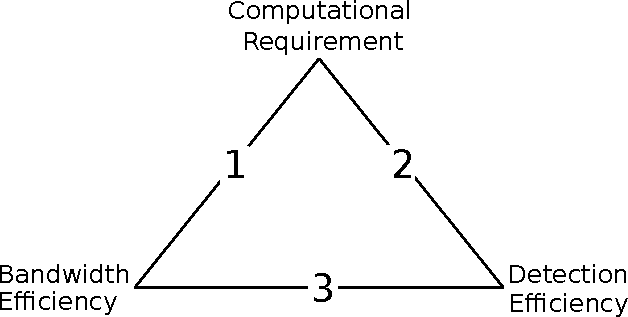
\includegraphics[width=0.5\linewidth]{img/edge_computing_vs.pdf}
    \caption{Comparison of the three event detection methodology across three metrics.
    Methods are as follows: naive method (2), self triggering (1), Napali, hybrid solution (3)}
    \label{intro:fig:edge}
\end{figure}
Figure \ref{intro:fig:edge} illustrates the strengths and weaknesses of the three approaches to anomaly detection.
The naive method provides the best detection ability and the smallest node computation requirement.
However, it does so at the cost of the largest bandwidth consumption.
The self triggering method has the lowest bandwidth consumption of the three.
The disadvantage of this method is twofold.
First, in order to maintain a high detection rate, a reasonably low threshold for anomalies has to be used.
This may cause a large number of false positives due to local noise and sensor noise.
Second, global anomalies will often diminish in magnitude as a function of distance from the epicenter, thus far removed sensor nodes may completely miss events.
These low threshold events may be invaluable for reconstructing the dynamic of the anomaly propagation, however they will be missed by the detection algorithms.


Napali's hybrid approach provides the opportunity for much better anomaly detection rate and background noise rejection, by correlating the features that are computed on the sensor nodes.
Napali has moderate bandwidth consumption, however the bandwidth consumption is tunable since the features can be computed for varied temporal windows, the length of which can be adjusted in real time.
Napali requires the highest sensor node computing power, since not only does it need to extract the triggering features from from raw data, it needs to maintain a buffer of sensor measurements to send to the sink if an anomaly is detected.

The main operational downside of the Napali framework, is the requirement for two way communication between the sink and the sensor node.
In order to participate in event detection Napali sensors need to be able to both send raw and feature extracted data, as well as receive the control signals from the sink.
In contrast, the naive and self triggered approaches only require a one way link to send the raw data to the sink.
As such, standalone devices can be retrofired to participate in distributed event detection in the naive and self triggered approaches, while Napali requires custom devices specifically tailored for cooperative event detection.

The advantages of the Napali methodology compared to the naive and self triggered approaches are enumerated below:
\begin{enumerate}
    \item \textbf{Bandwidth usage is minimized:} Instead of sending the entirety of raw data, only extracted features are sent.
    This features will have a tiny fraction of the bandwidth requirement when compared to raw waveforms.
    Furthermore, the temporal window which encompasses a single feature can be adjusted in real time.
    Thus as soon as an anomalous behavior is observed in a subset of sensors, this window can be adjusted for a finer grained feature extraction.

    \item \textbf{Effects of latency are minimized:} Even at 1Msample/second at 16bits of resolution, the memory requirement to store 5 minutes of raw waveform without compression are on the order of 512MB, which is well within the realm of cheap single board computers.
    With compression specifically suited to the signal of interest, the memory requirement can be reduced even further.
    This gives the triggering stream sink plenty of time to respond to the anomalies in the data and request raw waveform from the monitoring devices.

    \item \textbf{Sink processing requirements are minimized:} Since most of the feature extraction is already performed at the device level the triggering stream sink computational resources can be minimized.
    With the advent of IOT, the computational capacity of the edge devices is increasing.
    Napali exploits these resources, and thus minimizes the sink computational requirements.

    \item \textbf{Sub-threshold data acquisition is a cost-effective way to improve understanding of grid-local anomalies:}
    The triggering stream sink makes the decision to acquire raw waveform from sensor nodes.
    This allows researchers to collect data from devices which were only mildly affected or not affected by the disturbance.
    This provides new possibilities for investigation of disturbance propagation across the sensed area.
    Furthermore, subthreshold data acquisition from leaf node allows for monitoring of the internal system state.

    \item \textbf{Increased resiliency with respect to power failure:}
    In the case of the complete power failure or communication blackout, if the monitoring device has a battery backup capability, each sensor has a record of the entire raw waveform leading up to the power interruption.
    Prior to shutdown the sensor node will transfer all of the raw data from the volatile memory to on-board permanent storage.
    Once the power or communication channel is restored, select portions of the buffer may be sent back to the data sink.
    This creates an additional layer of resiliency for the anomaly detection network.

    \item \textbf{Increased flexibility with respect to privacy protection policies:} Anomalies which were only observed at a single point are most likely local noise and pose little value for global state monitoring.
    IIt can be up to the owner of each sensor node to decide how to process disturbances which affect their sensor.
    For example, a node owner may choose to record a full waveform, only certain features, or record nothing at all.
    Secondly, if the saturation of the device is high enough only a subset of them would need to send a triggering stream for event detection, while the rest will be used for acquiring raw waveform for small temporal regions containing global events.

    \item \textbf{Temporal locality allows Napali to provide improved insights into power quality anomalies over traditional triggering algorithms:} By exploiting the temporal locality it is possible to ascertain the geographical extent of the anomaly with only coarse features.
    This allows for a simple robust algorithm which may be deployed at the sink node for anomaly detection.
\end{enumerate}

\section{The problem of power quality} \label{intro:sec:pq}
Power quality monitoring, along with other smart grid domains is a field well suited for distributed sensor network monitoring.\cite{liu2017distribution} \cite{peisert2017lbnl} As the power grid moves from centralized generation with a few centralized power plants to distributed generation with residential power production, a distributed consumer level monitoring system becomes ever more important.
Traditionally, utilities do not monitor the quality of power besides the consumption beyond the substation level.
This is due to the fact that the last opportunity that the utility has to regulate and filter the grid voltage in the hierarchical power distribution is at the substation, or neighborhood level.
This methodology is unsustainable, as residential renewable energy production if not properly monitored and controlled will have an adverse effect on overall grid stability.
Furthermore, lack of residential monitoring may lead to dangerous conditions such as islanding, where an otherwise powered-down grid may have a small powered island sustained only by the unmonitored residential renewable generation.
Finally, residential power quality monitoring gives utility costumers an opportunity to evaluate the quality of power delivered to their household.
As consumer electronics are becoming more and more complex, they become more sensitive to the power anomalies.
Grid monitoring is traditionally the responsibility of the utility, however in most cases utilities only have to disclose power interruptions lasting several minutes.
Small interruptions, and partial interruptions such as voltage sags, swells, frequency fluctuations and transients will often go undisclosed by the utility and unnoticed by the consumer, but may cause premature failure in grid connected electronic devices.
It is in the best interest of the consumers to monitor the quality of the power that is delivered to them, meanwhile the same same monitoring system will also allows researchers and utilities to monitor the entirety of smart grid.

\begin{figure}[h]
    \centering
    \begin{subfigure}{.5\textwidth}
        \centering
        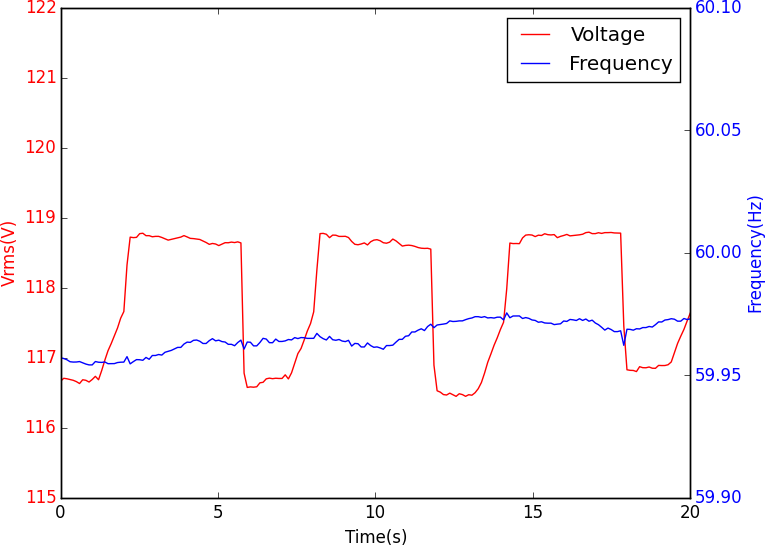
\includegraphics[width=0.9\linewidth]{img/hotplate.png}
        \caption{Voltage signal produced by a hotplate.}
        \label{intro:fig1:sub1}
    \end{subfigure}%
    \begin{subfigure}{.5\textwidth}
        \centering
        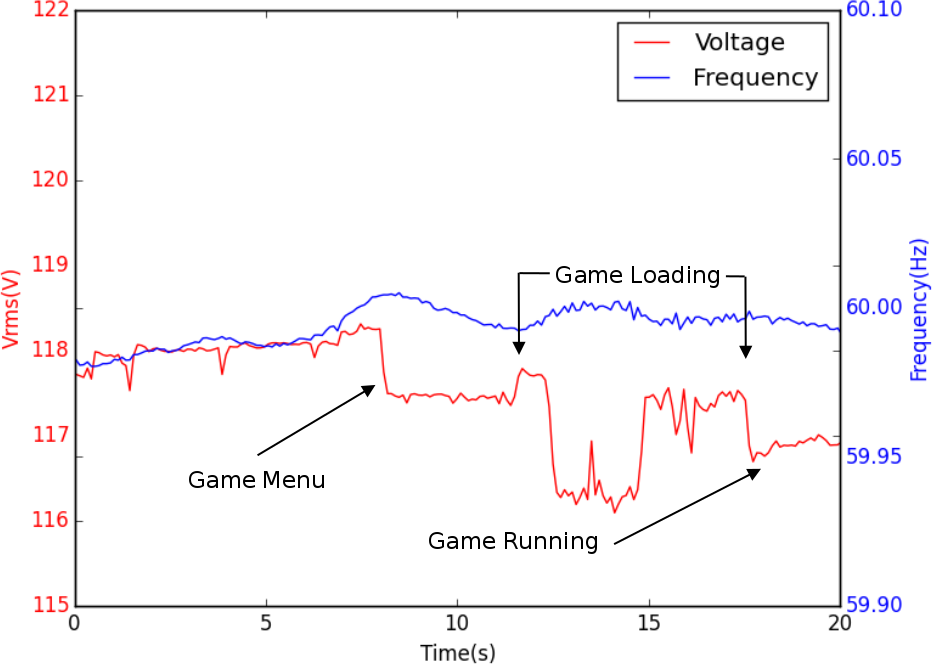
\includegraphics[width=0.9\linewidth]{img/PC.png}
        \caption{Voltage signal produced by a desktop PC running a complex task}
        \label{intro:fig1:sub2}
    \end{subfigure}

    \begin{subfigure}{1\textwidth}
        \centering
        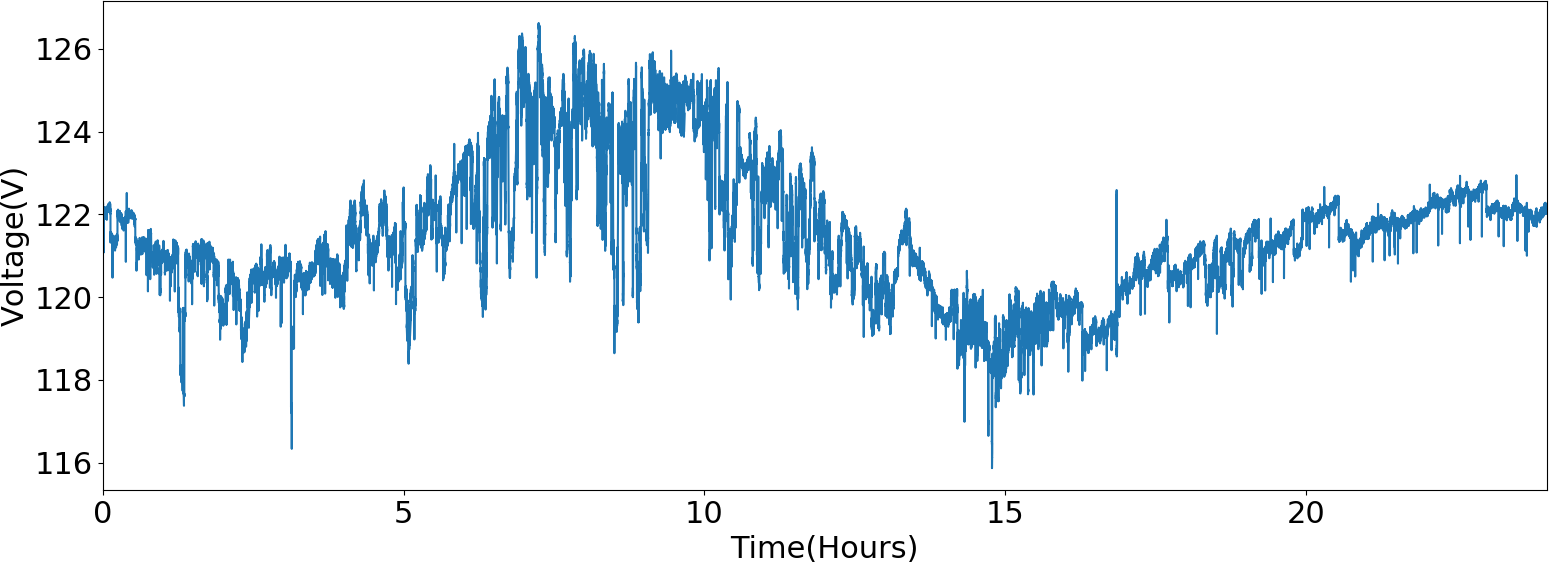
\includegraphics[width=0.9\linewidth]{img/johnson_daily.png}
        \caption{Line voltage recorded over 24 hours in a residential household with photovoltaic installation.}
        \label{intro:fig1:sub3}
    \end{subfigure}

    \caption{$v_{rms}$ waveform generated form the consumer side of the meter under various conditions.
    All waveform were recorded using the OPQ Box 2.}
    \label{intro:fig:1}
\end{figure}

Residential power quality monitoring presents a number of issues, as illustrated in Figure \ref{intro:fig:1}.
First of all, it is difficult to discern which ``side'' of the utility meter a power disturbance came from.
Is the origin of the disturbance within a building and flow outward through the meter into the grid, or did it originate elsewhere in the grid and flow into the building through the meter?
Consider a voltage sag generated by a 1kW hot plate shown in Figure \ref{intro:fig1:sub1}.
Since the output impedance of the power grid is non-zero, a high powered device can cause a significant voltage sag affecting every device connected to the same circuit.
Second, recoding the voltage waveform resulting from non-linear load can result in privacy leaks for the end user.
Consider the voltage waveform produced by a PC running a video game as shown in Figure \ref{intro:fig1:sub2}.
Throughout the game loading process, the power load varies based on which components are in use.
Furthermore, regions with CPU load, hard disk load and video card load can be readily identified by measuring the resulting voltage sag.
Recording these event's has an adverse effect on end-users privacy and offers no immediate benefit in studying grid stability.
Finally distributed power generation such as rooftop solar has significant effect on the residential voltage waveform.
Consider the voltage waveform shown in Figure \ref{intro:fig1:sub3}.
This waveform was recorded over 24 hours in a household with a rooftop photovoltaic installation.
Similar to the voltage sag case, since the power grid impedance is non-zero residential power generation will cause a voltage swell during peak hours of sunlight as evident by the waveform.
Combined with the global voltage sag during hours of peak demand (3pm) combined with the lack of PV production during that time, photovoltaics installations can result in a daily $10V_{rms}$ swing.
Residential power quality monitoring can be accomplished via a distributed sensor network made up of power quality monitoring devices with high degree of penetration across the end points of a power grid.
Furthermore, in order to monitor the dynamics of the entire power grid via residential line voltage monitoring, it is imperative to monitor across multiple locations simultaneously.
This combined with temporal and spatial correlations of data produced by the sensors provides the potential for identification of grid-wide anomalies without a high rate of false positives.
Additionally, not all power quality events affect the entire grid, due to the hierarchical structure of the power distribution.

\section{An edge computing approach to power quality monitoring.}\label{sec:edge-computing-approach-to-power-quality-monitoring.}

IEEE1159 standard describes the techniques for single location power quality monitoring.
For transient monitoring it suggests a sampling rate of at least 7680 samples/second, up to 1 Megasample/second.
This implies that if a power quality event detection system relies on raw data from all monitors((i.e. the naive method)) it would do so at a very large bandwidth cost.
At 20 Ksamples/second at 16bit per samples a single monitoring device would generate 300Kb/second.
Several thousand devices could easily saturate at 1Gb link with no obvious benefit.
Collecting and recording all of the raw waveform data from residential power quality meters for batch processing presents some privacy concerns as outlined above.
On the other hand, an on board event detection methodology, allows the measurement devices to select which temporal regions of measurements constitute an event.
This is a perfect strategy from the consumer's perspective, since it would allow for recording of power quality information which directly impact their residence.
As mentioned in Section \ref{intro:edge}, this method relies on a threshold based approach where every device has a computes several metrics from the raw waveform and compares then to preprogrammed threshold values.
Metrics such as $V_{rms}$, fundamental frequency and THD are easily adapted for single point power quality measurements.
Temporal regions during which these metrics surpass a threshold are considered by the device as a power quality event, and thus are recorded.


The problem with the self-triggered method is that grid-wide power quality events do not affect the entire grid in the same way.
For example, due to the grid's hierarchical structure, a voltage sag on one sub-circuit can manifest as as a sag of a different magnitude or even a swell on another.\cite{kahle2016power}
This may result in a situation where some of the monitoring devices will not consider a power quality anomaly as an event, because it did not surpass the metric threshold, and simply ignore it.
From the research perspective, however, it is important to get raw data from all of the affected devices not just, the ones that were the most affected.
This additional information could be used to localize the disturbance, as well as better evaluate it's impact.
This makes a hybrid centralized/decentralized event acquisition strategy more attractive for distributed residential power quality monitoring.
In this scheme all monitoring devices use local processing resources to feature extract the incoming waveforms while storing them locally for several minutes.
A sink collects all of the extracted features and looks for anomalies which are present in the feature data stream which we will refer to as the triggering stream.
If an anomaly is present in only a single device, it is highly probable that the disturbance occurred in the residence.
Depending on the user's privacy preference, raw data for a single device anomaly can be be recorded for later analysis, or in case of a highly privacy conscious user, ignored.
On the other hand, if the triggering stream shows an anomaly temporally collocated across multiple devices, the entire network or a subset of the network may be queried for raw waveform data for a temporal region which corresponds to the disturbance in the triggering stream.

The main disadvantage of this method is that while there are plenty of power quality event detection methodologies for single location, there has been little research into the distributed event detection methods and metrics.
The two problems are quite similar, indeed one may use the same metrics for distributed event detection as with the single point power quality monitoring.
However, it's also important to consider temporal locality of anomalies detected across multiple devices as well as the effects of device synchronization.
Power quality anomalies such as voltage sags and transients will propagate through the transmission lines at the speed of light, however due to the non-linear elements which make up the power-line junctions, a certain temporal spread in event detection across multiple locations is expected.
For large power grids such continental United States grids, large frequency fluctuations propagate in a highly nonlinear ways.
In these cases the event propagation is limited by the inherent rotational inertia of the power generation systems, and the speed at which the grid protection elements such as reclosers and circuit breakers operate.
Regardless, the closer local anomalies are detected in time, the more likely are they to be a result of a gridwide event.
Unfortunately, it is unfeasible to perfectly temporally synchronize the distributed power quality monitors.
While methods such as GPS can in principle provide synchronization of up to 10ns jitter across a large geographical region, they require a line of sight to the sky, and add a non-trivial cost to the bill of materials for every power quality meter.
Furthermore, GPS is prone to losing signal depending on atmospheric conditions, and can be very sensitive to fluctuations in the power supply voltage, a critical time in power anomaly detection.
An alternative to GPS is Network Time Protocol.
Network time protocol can provide timing synchronization on the order of $~10ms$ across Internet, which is on the order of $\frac{1}{2}$ of a grid cycle.
NTP performance could be further improved by using geographically close time servers which are themselves synchronized via GPS. Consider a situation where two devices are located in household which experience a local $100ms$ power quality disturbance every $10$ minutes.
Even with a $~10ms$ synchronization jitter, it will take on average $21.5$ days before the two disturbances are observed within $20ms$ of each other.
If a third device is introduced, it is highly unlikely that all 3 would observe unrelated local anomalies within $20ms$ of each other over the lifetime of the power quality monitoring network.
This implies that combination of temporal and threshold based correlation on the feature extraction data would allow one to build a robust residential based power grid monitoring system which would yield a very low rate of false positives.

\begin{figure}[h]
    \centering
    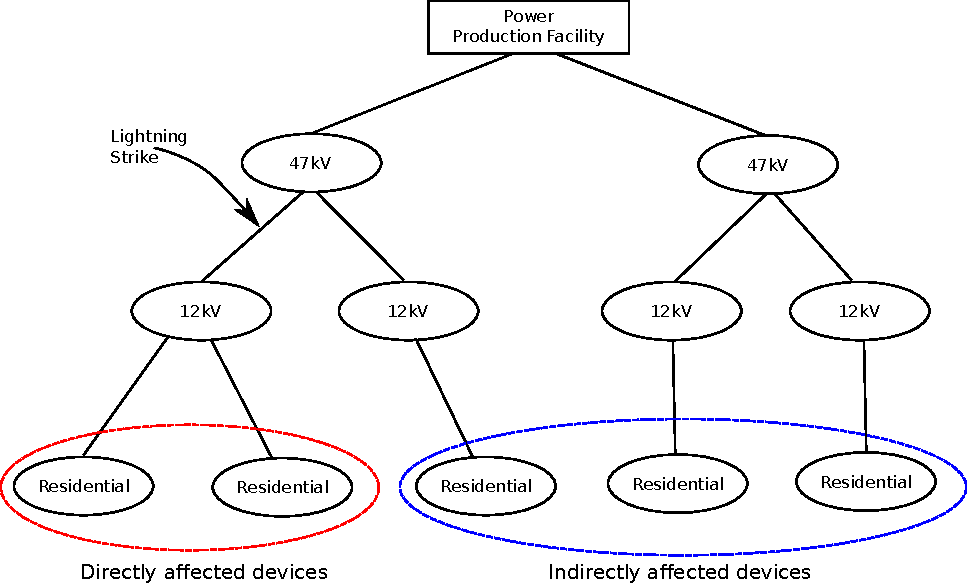
\includegraphics[width=0.9\linewidth]{img/grid_hierarchy_cartoon.pdf}
    \caption{Power quality anomaly propagation example.}
    \label{intro:fig2}
\end{figure}

\section{Thesis claim and evaluation} \label{intro:sec:claim}

Today's big data world is plagued with issues of data cleaning and validation, even though it's being increasingly relied on for timely, accurate and actionable intelligence.
With large ingress of unstructured data these issues are unavoidable, and preprocessing will remain a large portion of the analysis workload.
However, in the case of sensor networks designed for a specific purpose, the tasks of anomaly detection can be pushed to the edge of the network using the Napali methodology.

\begin{tcolorbox}
\textbf{The claim of this thesis is that Napali provides a novel architecture that is both a feasible solution to the problem of distributed power quality monitoring and provides significant benefits over the two standard alternative architectures (the self-triggered method, where all computation/storage is performed at the edge nodes, and the naive method, where all computation/storage at the occurs at the sink).
Furthermore, the Napali architecture can, in principle, provide benefits for other domains beyond power quality.}
\end{tcolorbox}
In order to evaluate the claim of this thesis, I implemented it as part of the Open Power Quality(OPQ) system and applied it to the problems of power quality monitoring.
Combined with higher level anomaly analysis, Napali provides important services for Open Power Quality power quality monitoring network.
This network is made up of a group of monitoring devices as well as a centralized data sink server.
This system was deployed for testing at the University of Hawaii at Manoa campus, by deploying power quality monitors across 15 University buildings.
The University of Hawaii at Manoa campus is a unique testbed for such a network, since the entire campus is isolated to its own microgrid, connected to the municipal Oahu grid via a 46kV feeder.
Furthermore, the University of Hawaii has deployed a set of smart power monitors at the key positions in the grid, which was used as a state-of-the-art ground truth for evaluation of OPQ performance.

The OPQ system relies on a custom residential power quality monitor called OPQ Box, designed specifically for distributed monitoring using the Napali framework.
Instead of performing local analysis on the voltage waveform with the aim of PQ anomaly detection, or forwarding all the recording measurements to the centralized sink, OPQ boxes computes a small subset of features on the input voltage waveform.
These features are then forwarded to the Napali framework's centralized sink which performs the anomaly detection on reduced data, while the raw waveform is retained for a short time on the OPQ Box.
If the sink determines that a possible anomaly has occurred, a request is sent to the affected and nearby devices for raw data.

The goal of Napali is not to provide a low rate of false positives for a particular type of a power quality disturbance.
Indeed, once the raw data is acquired by the sink, filtering through the potential anomalies is trivial using well established methods.
Instead, the focus of Napali is balancing the low bandwidth required for detection with a low rate of false negatives.
Furthermore, monitoring at the leaf notes relies on the hierarchical nature of the power grid in order to ascertain the state of the entire power generation and delivery system.
As noted in the literature, power quality disturbances tend to propagate down the hierarchy as shown in Figure \ref{intro:fig2}.


Consider a lightning strike on a hypothetical 12kV feeder line in a hierarchical power grid.
The directly affected devices will be the ones downstream from the disturbance.
These devices will experience the most severe effects, most notably transients, as they propagate throughput the power delivery infrastructure.
The indirectly affected devices will expedience a power anomaly mainly attributed to the power production entities trying to compensate for the large disturbance caused by the lightning strike.
Thus, monitoring of the leaf nodes of the power delivery system can in principle provide insights into the disturbances that originate deep inside the power distribution network.

The Open Power Quality system is designed to be a test bed for development of new power quality detection and analysis algorithms.
It can facilitate development of new techniques and methods for studying power system, by utilizing the Napali framework as the main anomaly detection methodology.
I assessed the data collected by the OPQ network at the University of Hawaii in order to determine if the claimed benefits of the architecture are observed in practice.


To reiterate: the central claim of this thesis is that Napali provides a feasible solution with significant benefits.
I will provide evidence for this central claim by evaluating the following subclaims about Napali:

\subsection{Napali minimizes bandwidth usage}\label{subsec:napali-minimizes-bandwidth-useage}
Bandwidth consumption of the OPQ system was be carefully monitored, recorded and compared to the bandwidth required to transmit the equivalent amount of raw data.
Furthermore, a Self-Triggered data acquisition ran along side the Napali event detector.
Thus, all three methods were compared in bandwidth utilization.
A more detailed description of this evaluation is found in Section \ref{subsec:napali-bandwidth-usage}.

\subsection{Napali mitigates device latency effects}\label{subsec:effects-of-latency-are-minimized:}
I examined the latency limits of the triggering system.
Latency effects on the Naive and Napali event detection methodologies were evaluated.
Since these limits are heavily dependent on the raw data storage ability of the OPQ Box, latency effects were tested under various amounts of memory allocated for this task.
A more detailed description of this evaluation is found in Section \ref{subsec:effects-of-latency-in-the-napali-framework}.

\subsection{Napali minimizes sink processing requirements}\label{subsec:napali-minimizes-sink-processing-requirements}
Synthetic benchmarks were carried out on the sink node to determine the scalability of the triggering system.
These scalability metrics were compared with a synthetic benchmark of running multiple copies of the OPQ Box analysis software on the same node.
This allowed me to compare the scalability of the sink node in the case of sending the entirety of raw data stream versus the Napali framework's approach of only sending extracted metrics.
A more detailed description of this evaluation is found in Section \ref{subsec:sink-processing-requirement-under-the-napali-framework}.

\subsection{Napali temporal locality triggering results in a low false negative detection}\label{subsec:temporal-locality-capabilities:}
Data acquired from the UH building level meters was compared with the data acquired via the Napali triggering framework.
This allowed me to establish the rate of false negatives and evaluate the temporal locality triggering algorithm.
A more detailed description of this evaluation is found in Section \ref{subsec:temporal-locality-triggering-of-the-napali-framework}.


\subsection{Sub-threshold data acquisition is a viable event detection strategy}\label{subsec:sub-threshold-data-acquisition:}
I examined a subset of events that can only be detected via the subtheshold triggering.
This was performed by analysing UH meter data, searching for events that Napali could only detect via subthreshold detection.
This provided a baseline comparison of Napali with a commercially deployed system.
A more detailed description of this evaluation is found in Section \ref{subsec:sub-threshold-data-acquisition}.

\subsection{Napali failure resiliency and flexible privacy}\label{subsec:napali-failure-resiliency-and-flexible-privacy}
Although power failure resiliency and flexible privacy are claimed benefits of the Napali architecture, they were not evaluated as part of this thesis research.
Flexible privacy required a much larger deployment, and a user study, which was beyond the scope of this project.
Evaluating the power failure resilience of the Napali framework would require a significant development effort for the battery management system.
Since complete power failures are quite rare, there is no guarantee that a single power outage would occur on the UH campus during the deployment.

\subsection{Napali in other domains}\label{subsec:napali-in-other-domains}
A final part of the central claim of this dissertation is that the Napali architecture can be applied to other domains.
Once the Napali framework was fully characterized, and its strengths and weaknesses were well understood, I performed a literature review of other domains which could benefit from Napali-like approach to event detection.
I further characterized the kinds of design changes to existing sensors that the Napali Framework required in order to apply it to these domains.
This work is can be found in Section \ref{sec:application-of-napali-in-other-domains}.
